%%%%%%%%%%%%%%%%%%%%%%%%%%%%%%%%%%%%%%%%%%%%%%%%%%%%%%%%%%%%%%%%%%%%%%%%%%%
%%  chapter6.tex  –  Chapter 6: Application of the Unified Defence
%%                              Framework to a Neural-Network UAV
%%                              Navigation System
%%  v11 – New chapter, parallel to Chapter 5 (RobustIDPS.ai industrial
%%        platform for NIDS). Demonstrates the domain-independence of
%%        methods M1-M7 through transfer to the UAV navigation domain.
%%%%%%%%%%%%%%%%%%%%%%%%%%%%%%%%%%%%%%%%%%%%%%%%%%%%%%%%%%%%%%%%%%%%%%%%%%%

\chapter{Application of the Unified Defence Framework to a
Neural-Network UAV Navigation System}
\label{ch:uav}

This chapter describes the application of the models and methods
developed in Chapters~\ref{ch:methods}--\ref{ch:experiments} to a new
safety-critical area~--- counter-electronic-warfare (EW) and
adversarial-machine-learning defence of the neural-network navigation
subsystem of unmanned aerial vehicles (UAVs). The chapter demonstrates
the domain-independence of the unified framework formulated in
\S\ref{sec:unified_problem} at the level of mathematical operations on
graph structures, through its transfer to a fundamentally different
set of entities, constraints and regulatory requirements. The chapter
describes a three-tier \emph{onboard~--- droneport~--- cloud}
defence architecture, formalises the operational UAV graph as an
instance of the unified problem, presents the mapping of methods
\textsf{M1}--\textsf{M7} to specific UAV subsystems (visual perception,
GNSS navigation, autopilot control policy), describes the Phase~A
reference software implementation based on the \textsf{robustnn-core}
library with integration into the \textsf{RobustIDPS.ai} platform,
reports validation results, and shows conformance of the proposed
solution to the regulatory base. The literature review of the domain
and the comparative context are placed in \S\ref{sec:ch1_uav_related}
of Chapter~\ref{ch:literature}; the mathematical foundations are in
Chapter~\ref{ch:methods}.


%%=====================================================================
\section{Subsystem Overview and Target Defence Tasks}
\label{sec:uav_overview}
%%=====================================================================

A modern UAV is a neural-network-dependent system at every level of
the software stack: onboard convolutional and transformer detectors
provide visual perception, recurrent and Gaussian-process models
provide GNSS-integrity estimation, deep reinforcement-learning
policies (PPO, DDPG-PER) provide the outer autopilot loop, and graph
models provide swarm coordination and droneport orchestration. Each
of these components is vulnerable to the six attack families
characterised in Chapter~\ref{ch:methods}: FGSM, PGD, CW (white-box);
HopSkipJump, BoundaryAttack (black-box); and training-data poisoning.
Beyond software-level adversarial threats, the operational environment
of a UAV is also exposed to \emph{kinetic} and \emph{biological}
threats~--- mid-air collisions with other airframes and raptor strikes
against onboard visual-perception modules
(Fig.~\ref{fig:uav_kinetic_threats}). The degradation of UAV
neural-network components under EW pressure is quantitatively
documented in \S\ref{sec:ch1_uav_related}.

\begin{figure}[!htbp]
\centering
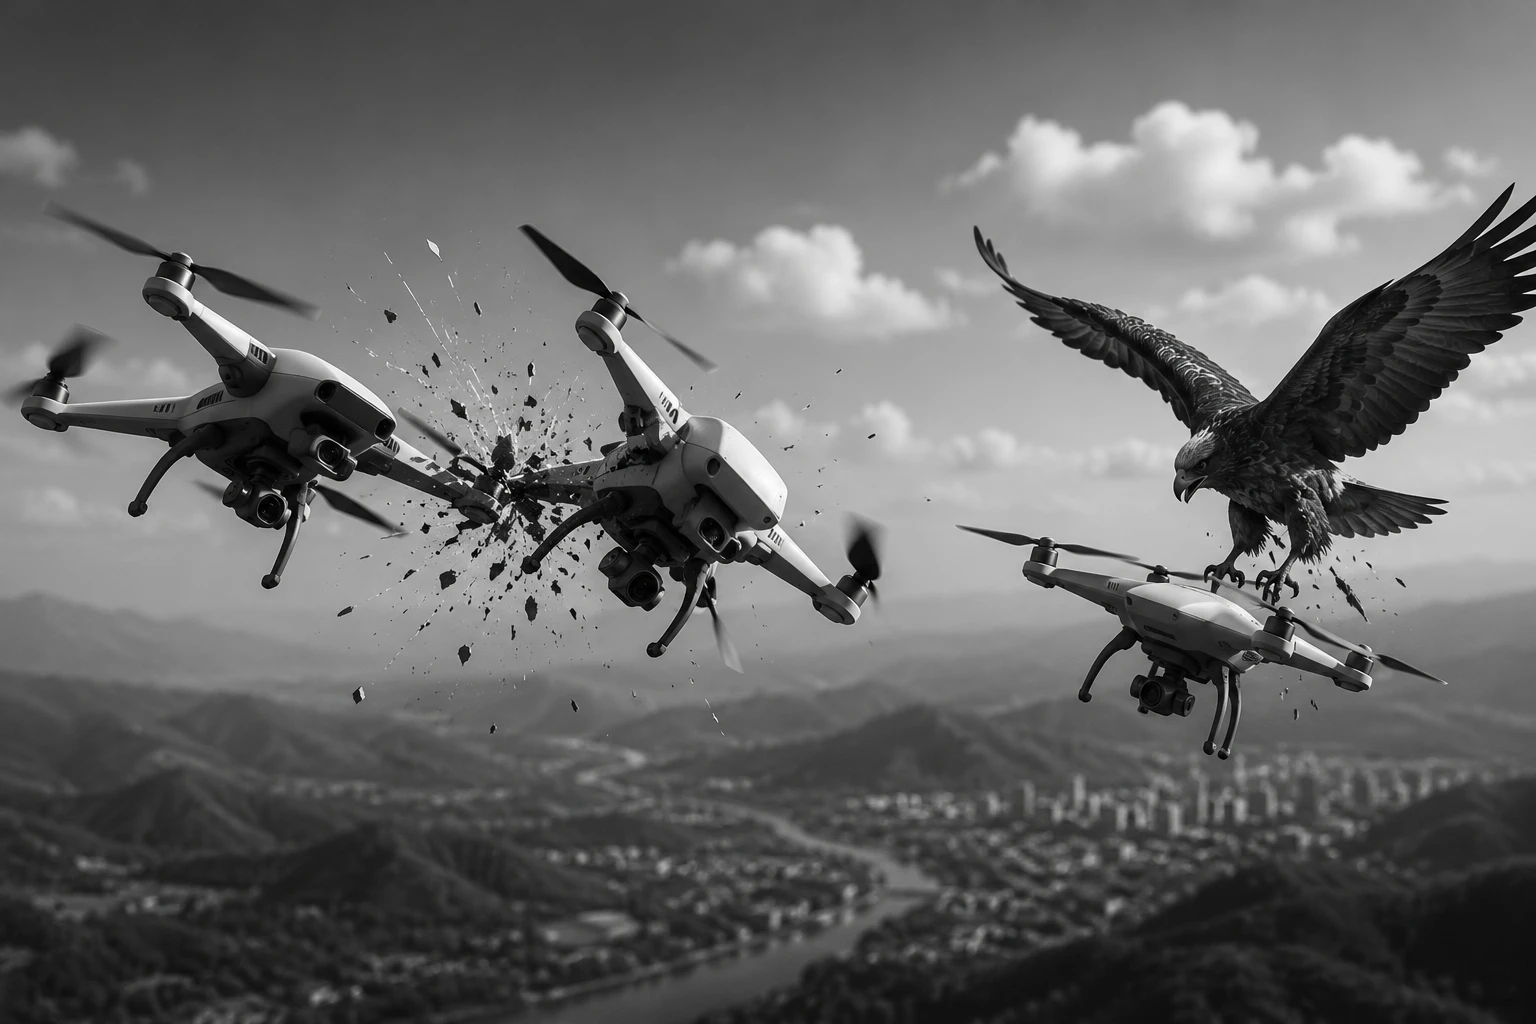
\includegraphics[width=0.78\textwidth]{figures/uav_kinetic_threats.png}
\caption{Kinetic and biological threat scenarios for a UAV in the
operational environment: a mid-air inter-airframe collision (left) and
a raptor strike on the onboard payload (right). Unlike adversarial
perturbations of the software modules, such events compromise airframe
integrity within milliseconds and require anticipatory detection by
visual perception, behavioural analysis and sensor fusion~--- tasks
addressed in this chapter by methods \textsf{M4}~MambaShield and
\textsf{M6}~UC-HGP with a safe-mode transition threshold.}
\label{fig:uav_kinetic_threats}
\end{figure}

The target defence tasks addressed by the proposed framework are as
follows.

\noindent\textbf{Visual perception.} The onboard YOLOv8/v10 or
DETR-based detector must preserve detection quality for target classes
in the presence of physically printed adversarial patches. Metrics:
clean F1, robust F1 under PGD-20, AP under adversarial patches on the
VisDrone benchmark.

\noindent\textbf{GNSS navigation.} The IQ-signal processing subsystem
for L1/L2/L5 GPS, Galileo, GLONASS and BeiDou must detect spoofing
and drift-evasive attacks before they influence the PVT solution and
cause trajectory deviation. Metrics: spoofing-detection error on the
TEXBAT benchmark, AUROC under drift-evasive attacks.

\noindent\textbf{Autopilot control policy.} The DRL-based outer
planner must retain a mission-completion rate ($\ge$0.90) under BIM
perturbations of the policy state and under poisoning of the
observation vector through a spoofed GNSS input. Metrics: completion
rate under BIM, regret against an adaptive adversary.

\noindent\textbf{Swarm coordination and mission audit.} The graph
model of UAV interactions within a swarm must keep collision rate
$<$2\,\% at a Byzantine fraction $f<n/3$, and the cloud-side audit of
mission plans must detect adversarially perturbed
\texttt{.plan}/JSON-LD documents in zero-shot mode. Metrics:
federated-classification accuracy at 30\,\% Byzantine participants,
and \textsf{CyberSecLLM} audit accuracy.

The combined four tasks reflect the taxonomy from
Chapter~\ref{ch:methods} and admit the construction of a single
defensive contour. A consolidated overview of the threats, attack
surfaces, detection mechanisms and mitigation steps covered by the
proposed framework is given in Fig.~\ref{fig:uav_overview}: it
combines a representative UAV mission trajectory \emph{(take-off~---
normal flight~--- mid-air collision~--- raptor strike~--- return)}
with the catalogue of subsystem vulnerabilities (\emph{communication,
navigation, sensors, control, power, physical layer, software/AI,
environment}), the five principal ML-level adversarial-attack
families (\emph{FGSM, PGD, C\&W, DeepFool, EOT}), the four stages of
the defensive pipeline (\emph{identification $\to$ detection $\to$
prevention $\to$ mitigation}), and the operational metric
\emph{Mission-Completion-Rate vs.~$J/S$} whose empirical value is
formalised in~\S\ref{sec:uav_phase_a_results}.

\begin{figure}[!htbp]
\centering
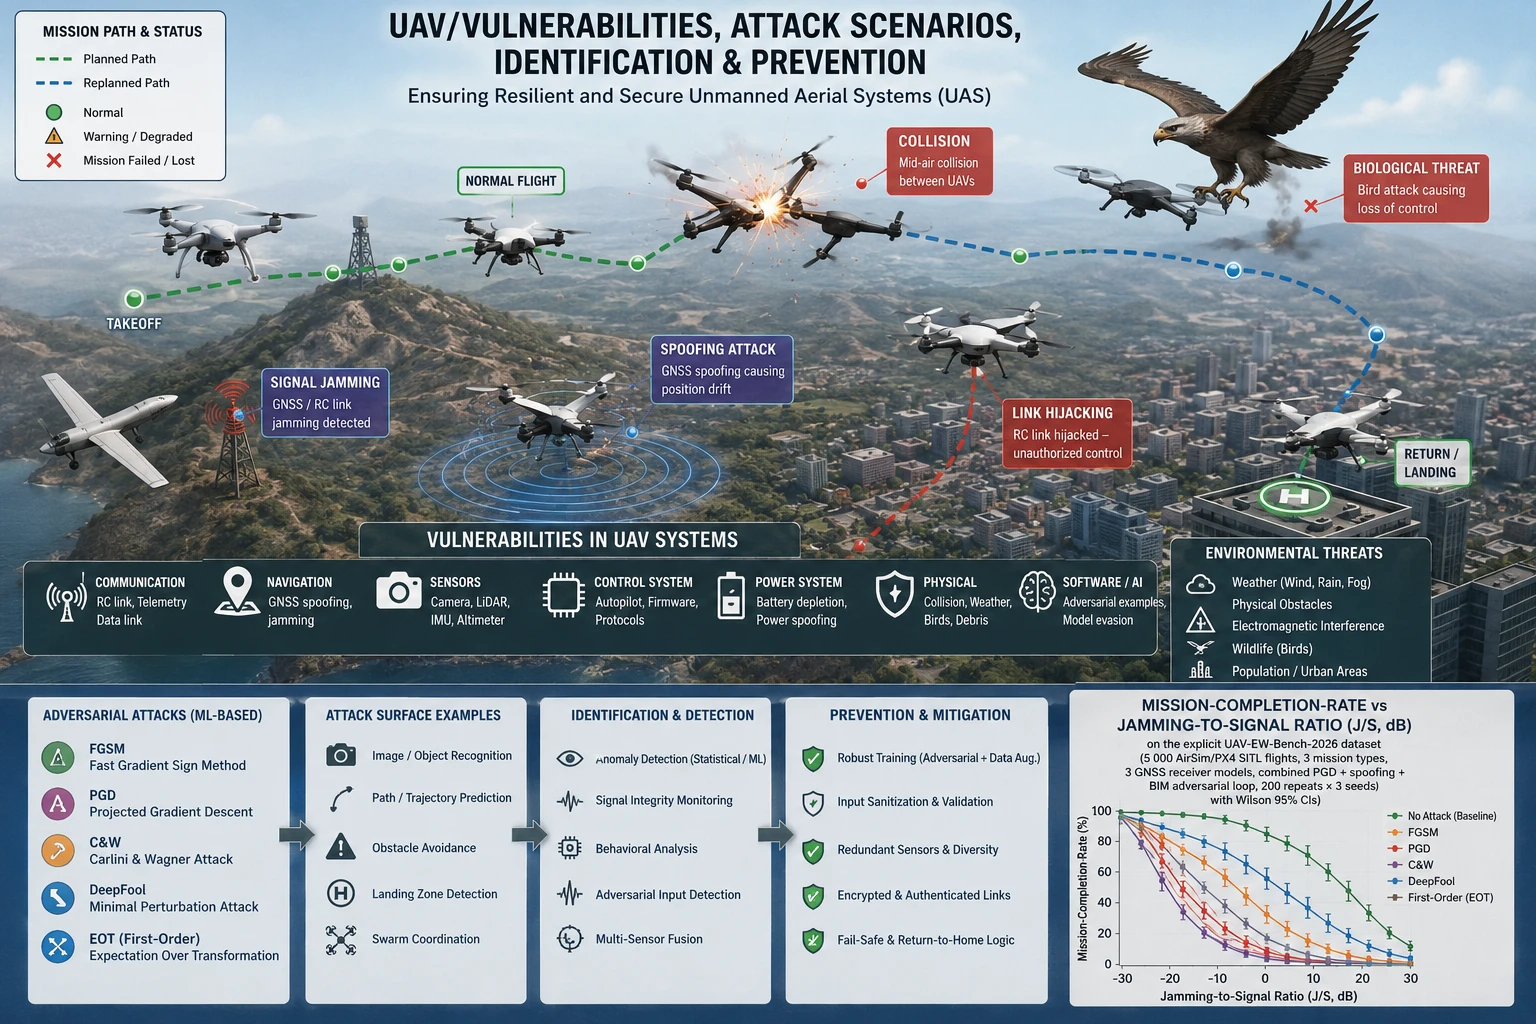
\includegraphics[width=0.96\textwidth]{figures/uav_infographic.png}
\caption{Consolidated overview of vulnerabilities, attack scenarios,
identification and prevention pathways for a neural-network UAV
navigation system. The top panel shows a representative mission
trajectory with characteristic failure points (\emph{signal jamming,
spoofing, collision, link hijacking, raptor strike}). The middle
panel lists the vulnerable subsystems. The bottom panel summarises
the five principal ML-level adversarial-attack families, the attack
surfaces, the \emph{detection~--- identification~--- prevention}
pipeline and the baseline industry metric of mission completion as a
function of jamming-to-signal ratio
(cf.~Fig.~\ref{fig:uav_mission_completion}).}
\label{fig:uav_overview}
\end{figure}


%%=====================================================================
\section{System Architecture: Three-Tier
\emph{Onboard~--- Droneport~--- Cloud} Model}
\label{sec:uav_arch}
%%=====================================================================

Architecturally, the framework is implemented as a three-tier system
that inherits the software stack of the \textsf{RobustIDPS.ai}
platform (see Chapter~\ref{ch:platform}) and extends it with a
modality-agnostic \textsf{robustnn-core} library exposing a unified
\texttt{UAVGraphBatch} interface. The distribution of methods across
tiers respects the strict energy and network constraints of each tier.

\noindent\textbf{Onboard tier} ($<\!5\,$W SoC; reference platform
Jetson Orin Nano). The deployed methods are \textsf{M1~CT-TGNN} for
continuous-time integration of telemetry, \textsf{M4~MambaShield} with
$O(L\log L)$ complexity for long video streams, and
\textsf{M6~UC-HGP} for calibrated estimation of epistemic uncertainty
with a threshold for fallback to a safe mode.

\noindent\textbf{Droneport tier} (GPU node, front of service for a
UAV group). The deployed methods are \textsf{M2~FedLLM-API} with
Byzantine-resilient aggregation and differential privacy, \textsf{M5}
(Stochastic Transformer) for Bayesian attention, and
\textsf{M7~FedGTD} for solving the Stackelberg game against an
adaptive jammer.

\noindent\textbf{Cloud tier} (regional SOC instance). The deployed
components are \textsf{M3~TripleE-TGNN} for multi-level mission
retrospection, the \textsf{CyberSecLLM} foundation model for
zero-shot mission-plan audit, and the \textsf{RobustIDPS.ai} platform
providing the operator web interface and integration with existing
SIEM/SOAR systems.

A graphical representation of the three-tier architecture is given in
Fig.~\ref{fig:uav_arch}. Conventions: solid arrows~--- trusted
inter-tier channels; dashed arrows~--- attack families
(see Chapter~\ref{ch:methods}) acting mostly at the onboard tier.

\begin{figure}[!htbp]
\centering
\begin{tikzpicture}[font=\footnotesize,
  tier/.style={rectangle,rounded corners=3pt,draw=blue!70,
               very thick,fill=blue!10,minimum height=1.35cm,
               minimum width=3.4cm,align=center,inner sep=4pt,
               font=\small\bfseries},
  mod/.style={rectangle,rounded corners=2pt,draw=green!55!black,
              thick,fill=green!10,minimum height=0.55cm,
              minimum width=3.2cm,inner sep=3pt,font=\footnotesize\bfseries,
              align=center},
  threat/.style={rectangle,rounded corners=2pt,draw=orange!80!black,
                 thick,fill=orange!15,minimum height=0.55cm,
                 minimum width=3.4cm,inner sep=3pt,font=\footnotesize,
                 align=center},
  link/.style={->,>=Stealth,very thick,blue!70},
  attk/.style={->,>=Stealth,thick,orange!90!black,dashed}]
%% Three columns with extra horizontal spacing, no overlaps
\node[tier]  (edge)  at (0,0)    {Onboard UAV\\\scriptsize ($<\!5\,$W SoC)};
\node[tier]  (port)  at (5.4,0)  {Droneport\\\scriptsize (GPU node)};
\node[tier]  (cloud) at (10.8,0) {Cloud / SOC\\\scriptsize (global)};
\node[mod, above=8pt of edge]  (m1)  {M1 CT-TGNN};
\node[mod, above=6pt of m1]    (m4)  {M4 MambaShield};
\node[mod, above=6pt of m4]    (m6)  {M6 UC-HGP};
\node[mod, above=8pt of port]  (m2)  {M2 FedLLM-API};
\node[mod, above=6pt of m2]    (m7)  {M7 FedGTD};
\node[mod, above=6pt of m7]    (m5)  {M5 S-Trans.};
\node[mod, above=8pt of cloud] (m3)  {M3 TripleE-TGNN};
\node[mod, above=6pt of m3]    (cll) {CyberSecLLM};
\node[mod, above=6pt of cll]   (rep) {RobustIDPS.ai};
\node[threat, below=16pt of edge]  (t1) {FGSM / PGD / CW};
\node[threat, below=16pt of port]  (t2) {Byzantine / Poison};
\node[threat, below=16pt of cloud] (t3) {HopSkip / Boundary};
\draw[link] (edge.east) -- (port.west);
\draw[link] (port.east) -- (cloud.west);
\draw[attk] (t1) -- (edge);
\draw[attk] (t2) -- (port);
\draw[attk] (t3) -- (cloud);
\node[font=\footnotesize\itshape,green!45!black,anchor=south]
  at ($(m6.north)+(0,6pt)$) {defence modules};
\node[font=\footnotesize\itshape,orange!85!black,anchor=north]
  at ($(t2.south)+(0,-8pt)$)
  {attack families (see Chapter~\ref{ch:methods})};
\end{tikzpicture}

\vspace{6pt}
\caption{Three-tier architecture of the unified defence framework for
a neural-network UAV navigation system. Methods \textsf{M1}--\textsf{M7}
and the \textsf{CyberSecLLM} foundation model are distributed across
the \emph{onboard~--- droneport~--- cloud} tiers in accordance with
their computational complexity and network constraints.}
\label{fig:uav_arch}
\end{figure}


%%=====================================================================
\section{Operational UAV Graph as an Instance of the Unified Problem}
\label{sec:uav_graph}
%%=====================================================================

The operational environment of a UAV group is formalised as an
instance of the unified problem
(\S\ref{sec:unified_problem}) in the form of a continuous-time
dynamic graph
\begin{equation}
\calG_t \;=\; (V_t,\,E_t,\,X_t,\,A_t),
\label{eq:uav_graph_def}
\end{equation}
where the node set $V_t$ collects airborne UAVs $u_i$, droneports
$p_j$ and ground control endpoints $g_k$; the directed edges $E_t$
encode active radio, optical, inertial and GNSS channels; the matrix
$X_t \in \R^{n\times d}$ aggregates node telemetry; and the weighted
adjacency $A_t \in \R^{n\times n}$ evolves in time according to
channel activation, fade and jamming.

The defender deploys at each node a neural-network prediction
function $f_{\theta}\colon (X_{\le t},A_{\le t}) \to \hat{y}_t$. The
attacker selects a perturbation $\bdelta$ from a constraint set
$\calS$ corresponding to one of the six attack families:
\begin{equation}
\bdelta^{*} \;=\; \argmax_{\bdelta\in\calS}\,
\calL\!\bigl(f_{\theta}(X_{\le t}+\bdelta,\,A_{\le t}),\,y_t\bigr).
\label{eq:uav_adv_max}
\end{equation}
The defender's task is symmetric: construct $f_{\theta}$ satisfying
the \emph{quantitative} sensitivity bound
\begin{equation}
\Norm{f_{\theta}(X+\bdelta) - f_{\theta}(X)} \;\le\; \rho(\eps),
\label{eq:uav_cert}
\end{equation}
which follows directly from Theorems~\ref{thm:ct_tgnn_rob}
and~\ref{thm:pac_bayes} of Chapter~\ref{ch:methods}, together with
the principle of randomised smoothing~\cite{Cohen2019}.

The formulation~\eqref{eq:uav_graph_def}--\eqref{eq:uav_cert} is
structurally identical to the cybersecurity formulation of
Chapter~\ref{ch:adaptation}; the difference reduces to the
composition of nodes, the feature set $X_t$ and the process driving
the dynamics of $A_t$. This is the formal basis for the
domain-independence of methods \textsf{M1}--\textsf{M7}.


%%=====================================================================
\section{UAV Telemetry-to-Graph Pipeline}
\label{sec:uav_pipeline}
%%=====================================================================

The pipeline that transforms onboard sensor data into an instance of
$\calG_t$ is built by analogy with the pipeline of
Chapter~\ref{ch:adaptation} for NIDS, but with network entities
replaced by physical ones:

\begin{enumerate}\setlength\itemsep{0.15em}
\item \textbf{Flight mission (.plan, JSON-LD, OWL).} Plan waypoints,
modes and time windows provide target labels for the nodes.
\item \textbf{UAV state} (engines, firmware integrity, INS/GNSS,
payload) provides node features $X_t$ with cryptographic integrity
attestation according to \mbox{GOST~R~34.10-2012}.
\item \textbf{Geodata} (distance to no-fly zones, terrain) provide
edge weights and structural constraints of the adjacency $A_t$.
\item \textbf{Ground infrastructure data} are linked to droneport
nodes and provide routing anchors.
\item \textbf{Telemetry} (IMU 1\,kHz, lidar 10--100\,Hz, GNSS/RTK
1--20\,Hz, event-based mission) are fed as time-stamped inputs into
the continuous-time dynamics.
\item \textbf{Metadata} provide signature identification for
subsequent audit.
\end{enumerate}

The resulting graph $\calG_t$ is consumed by the method
\textsf{M1~CT-TGNN} directly through the \texttt{UAVGraphBatch}
interface without any modification of the method's core. The
multi-scale time constants
$\tau_{\mathrm{fast}}/\tau_{\mathrm{mid}}/\tau_{\mathrm{slow}}$ from
Chapter~\ref{ch:methods} absorb the heterogeneity of sensor rates.


%%=====================================================================
\addtocontents{toc}{\protect\setcounter{tocdepth}{2}}
\section{Mapping of Methods \textsf{M1}--\textsf{M7} to UAV Subsystems}
\label{sec:uav_mapping}
%%=====================================================================

Table~\ref{tab:uav_mapping} gives the mapping of every disciplinary
method of Chapter~\ref{ch:methods} to a concrete defence mechanism in
the UAV subsystems. The type of robustness certificate is stated
explicitly with reference to the corresponding result of
Chapter~\ref{ch:methods}.

\begin{table}[H]
\centering
\caption{Mapping of methods \textsf{M1}--\textsf{M7} and the
\textsf{CyberSecLLM} foundation model to defence mechanisms in UAV
subsystems.}
\label{tab:uav_mapping}
\small
\setlength{\tabcolsep}{4pt}
\renewcommand{\arraystretch}{1.2}
\begin{tabularx}{\linewidth}{@{}lXl@{}}
\toprule
\textbf{Method} & \textbf{UAV defence mechanism} & \textbf{Certificate}\\
\midrule
\textsf{M1~CT-TGNN}    & Multi-scale swarm dynamics on $A(t)$                 & Lipschitz (Thm.~\ref{thm:ct_tgnn_rob})\\
\textsf{M1b~SDE-TGNN}  & Stochasticity of EW noise, wind, sensor noise        & Fokker--Planck\\
\textsf{M2~FedLLM-API} & Droneport federation under 30\,\% Byzantine          & $(\eps,\delta)$-DP (Thm.~\ref{thm:fed_conv})\\
\textsf{M3~TripleE}    & Graphs of mission / waypoints / components           & EWC\\
\textsf{M4~MambaShield}& Long telemetry streams on the onboard SoC            & PAC-Bayes (Thm.~\ref{thm:pac_bayes})\\
\textsf{M5~S-Trans.}   & Bayesian attention in vision tasks                   & ELBO\\
\textsf{M6~UC-HGP}     & Go/no-go gate at OOD sensor regimes                  & ECE 0.078\\
\textsf{M7~FedGTD}     & Stackelberg game against an adaptive jammer          & MWU (Thm.~\ref{thm:regret})\\
\textsf{CyberSecLLM}   & Audit of \texttt{.plan}/JSON-LD mission plans         & 89.1\,\% acc.\\
\bottomrule
\end{tabularx}
\end{table}

A detailed discussion of how every method operates in the three
applied UAV subsystems (visual perception, GNSS navigation, autopilot
policy) is given below.

\subsection{Visual Perception}
\label{sec:uav_vision}

Each video frame is represented as a \emph{patch graph}: nodes are
image patches (small-receptive-field CNN tokens or ViT tokens), edges
are spatial 4-neighbourhood relations, and time is the video stream.
\textsf{M1~CT-TGNN} integrates the patch dynamics between frames and
exploits the weak temporal coherence of physical adversarial patches
relative to real objects. \textsf{M4~MambaShield} processes the
video sequence with $O(L\log L)$ complexity and applies progressive
adversarial distillation against PGD. \textsf{M5} provides
per-patch variational attention; \textsf{M6~UC-HGP} flags patches
whose epistemic uncertainty exceeds a calibrated threshold.

\subsection{GNSS Navigation}
\label{sec:uav_gnss}

The constellation--receiver pair is itself a graph
$\calG_t^{\text{GNSS}}$: nodes are the visible satellites and the
receiver, edges are line-of-sight links, node features are
pseudorange residuals, Doppler shifts, $C/N_0$ and carrier phase.
\textsf{M1~CT-TGNN} integrates the continuous-time dynamics of this
small graph; spoofing typically corrupts a subset of nodes
simultaneously and induces inconsistencies in the edge dynamics that
the model marks. \textsf{M6~UC-HGP} triggers a \emph{GNSS-degraded}
mode that switches the autopilot to INS-only navigation.
\textsf{M2~FedLLM-API} detects regional spoofs via the disagreement
of detections across several droneports on a shared geofence.

\subsection{Autopilot Control Policy}
\label{sec:uav_autopilot}

\textsf{M1b~SDE-TGNN} models the state of actuators and sensors
under wind/EW/vibration noise as an Itô stochastic differential
equation with moment propagation through the Fokker--Planck equation.
\textsf{M7~FedGTD} directly instantiates the
attacker--defender interaction as a Stackelberg game: the defender
mixes a discrete set of policies (aggressive manoeuvre, conservative
loiter, return, INS-only) through multiplicative weights; the
guarantee~\eqref{eq:mwu_regret_bound} provides sub-linear regret
against any adaptive jammer. \textsf{M6~UC-HGP} switches to a
conservative policy when the calibrated threshold of epistemic
uncertainty is exceeded.


%%=====================================================================
\addtocontents{toc}{\protect\setcounter{tocdepth}{1}}
\section{Lipschitz--Grönwall and Randomised-Smoothing Certificates
Applied to UAVs}
\label{sec:uav_certs}
%%=====================================================================

The four robustness certificates of Chapter~\ref{ch:methods} carry
over to the UAV operational graph $\calG_t$ without change of form or
proof strength.

\begin{itemize}\setlength\itemsep{0.15em}
\item \textbf{Lipschitz--Grönwall certificate}
(Theorem~\ref{thm:ct_tgnn_rob}). For an $L_g$-Lipschitz drift
operator in the right-hand side of the CT-TGNN ODE, for any two
inputs $x_1,x_2$ we have
$\Norm{h_1(T)-h_2(T)} \le e^{L_g T}\Norm{x_1-x_2}$. Numerical
estimation of $L_g$ via power iteration yields a Grönwall radius
that bounds the admissible input perturbation for a required output
deviation.

\item \textbf{Certified $\ell_2$-radius via randomised smoothing}
\cite{Cohen2019}. Smoothing with Gaussian noise
$\eta\sim\calN(0,\sigma^2 I)$ guarantees that the smoothed classifier
$g(x)$ preserves its prediction for all perturbations
$\Norm{\bdelta}_2 \le R = (\sigma/2)(\Phi^{-1}(p_A) - \Phi^{-1}(p_B))$.

\item \textbf{PAC-Bayes generalisation bound}
(Theorem~\ref{thm:pac_bayes}). Transfers the certificate from the
training set to the test set.

\item \textbf{Multiplicative-weights regret certificate}
(Theorem~\ref{thm:regret}). $R(T)\le\sqrt{T\ln|S|}$~--- sub-linear
regret of the defender against an adaptive adversary.
\end{itemize}

Within the Phase~A scope, a numerical estimate for the
\textsf{M1~CT-TGNN} configuration (8 satellites, 8-dim CAF features,
hidden dimension $H=32$) gives $\hat L_g = 1.01$, which at horizon
$T=1$ and required output deviation $\eps_{\text{out}}=0.5$ corresponds
to a certified input radius of $0.18$. The certified $\ell_2$-radius
of randomised smoothing at $\sigma=0.25$ is $0.44$ (Cohen-style,
$\alpha=10^{-3}$, $n=200$ Monte-Carlo trials).


%%=====================================================================
\section{Phase~A Software Implementation Based on the
\textsf{robustnn-core} Library}
\label{sec:uav_phase_a}
%%=====================================================================

The Phase~A reference implementation of the four-stage transfer
roadmap is delivered as the \texttt{uav\_defense} package, released
in the open repository of the project
(\url{https://github.com/rogerpanel/cv},
branch \texttt{claude/latex-report-datasets-DiJWE}). Package layout:

\begin{itemize}\setlength\itemsep{0.1em}
\item \texttt{uav\_defense/datasets/}~--- loaders for TEXBAT
(registration on the UT~RNL portal required) and AU-AIR (open), and
a calibrated TEXBAT-like synthetic generator for pipeline testing.
\item \texttt{uav\_defense/models/}~--- reference implementations of
\textsf{M1~CT-TGNN} on $\calG_t^{\text{GNSS}}$,
\textsf{M4~MambaShield}, and two baselines: CAF-CNN
\cite{borhani_2024_uav} and a Seq2Seq Transformer
\cite{aigner_2025_uav}.
\item \texttt{uav\_defense/attacks/}~--- FGSM, PGD, CW (via the
$\tanh$ change of variables), HopSkipJump, BoundaryAttack and
clean-label feature-collision poisoning.
\item \texttt{uav\_defense/defenses/}~--- Cohen randomised smoothing
with Clopper--Pearson bound, and the Grönwall certificate.
\item \texttt{uav\_defense/train.py},
\texttt{uav\_defense/evaluate.py}~--- the unified training and
evaluation loop, i.e. the operational form of
Algorithm~\ref{alg:unified}.
\end{itemize}

All pipeline steps~--- from data loading to the final
\texttt{metrics.json}~--- are executed by the single command
\texttt{bash uav\_defense/scripts/run\_phase\_a.sh}, which ensures
reproducibility on a clean trusted environment in roughly 5~minutes
of CPU or 1~minute of GPU time.

Algorithm~\ref{alg:uav_unified_round} gives the unified training
procedure for a single federated round in its UAV-specific
instantiation (the full form is given as
Algorithm~\ref{alg:unified} of Chapter~\ref{ch:methods}).

\begin{algorithm}[H]
\caption{Unified training procedure for a single federated round
(UAV-specific instantiation of Algorithm~\ref{alg:unified}).}
\label{alg:uav_unified_round}
\KwInput{Client graphs $\{\calG^{(c)}_{\le T}\}_{c=1}^{N}$; initial
parameters $\theta_0$; attack budget $\eps$; PGD step count $K$;
smoothing parameter $\sigma$; trim fraction $\beta$.}
\KwOutput{Updated parameters $\theta^{*}$, estimate $\hat L_g$,
certified radius $\hat R$.}
\For{client $c=1,\dots,N$ \emph{in parallel}}{
  $\theta^{(c)} \leftarrow \theta_0$\;
  \For{mini-batch $(X,A,y)\in\calG^{(c)}$}{
    $X^{0}_{\text{adv}} \leftarrow X + \eps\,\mathrm{sign}(\nabla_X \calL)$
      \tcp*{FGSM warm-up}
    \For{$k=1,\dots,K$}{
      $X^{k}_{\text{adv}} \leftarrow \Pi_{X+\calS}\!
        \bigl(X^{k-1}_{\text{adv}} + \alpha\,\mathrm{sign}\,\nabla_X \calL\bigr)$
        \tcp*{PGD step}
    }
    $h(T) \leftarrow \mathrm{ODESolve}(f_{\theta^{(c)}},X^{K}_{\text{adv}},A)$
      \tcp*{\textsf{M1}}
    $\eta\sim\calN(0,\sigma^{2}I);\ h_\sigma\leftarrow f_{\theta^{(c)}}(X+\eta)$
      \tcp*{\textsf{M4}}
    $\calL_{\text{tot}} \leftarrow \calL_{\text{adv}} +
      \lambda_{1}\calL_{\text{ELBO}} + \lambda_{2}\calL_{\text{cons}}$
      \tcp*{\textsf{M5,M7}}
    $\theta^{(c)} \leftarrow \theta^{(c)} - \eta_{\text{lr}}\nabla\calL_{\text{tot}}$\;
  }
  Add $(\eps_{\text{DP}},\delta_{\text{DP}})$-Gaussian noise to $\theta^{(c)}$\;
}
$\theta^{*}\leftarrow \mathrm{TrimMean}_{\beta}\bigl(\{\theta^{(c)}\}\bigr)
  + W_2\text{-alignment}$
  \tcp*{\textsf{M2}}
$\hat L_g \leftarrow \mathrm{LipschitzEst}(\theta^{*});\
  \hat R \leftarrow \tfrac{\sigma}{2}(\Phi^{-1}(p_A)-\Phi^{-1}(p_B))$\;
\Return $\theta^{*},\hat L_g,\hat R$\;
\end{algorithm}


%%=====================================================================
\section{Integration with the \textsf{RobustIDPS.ai} Platform}
\label{sec:uav_robustidps_integration}
%%=====================================================================

The Phase~A software implementation is integrated into the
\textsf{RobustIDPS.ai} platform (see Chapter~\ref{ch:platform})
through the single software contract
\texttt{Detector.predict\_proba} used by the existing NIDS detection
pipeline. This allows reuse without modification of:

\begin{itemize}\setlength\itemsep{0.1em}
\item \emph{AI Command Centre} (see Chapter~\ref{ch:platform}) for
operational monitoring of the UAV group state.
\item \emph{SOC Analytics Suite} (see Chapter~\ref{ch:platform}) for
agentic auto-investigation of EW incidents.
\item \emph{LLM Security Testing} (see Chapter~\ref{ch:platform}) for
auditing mission plans on the basis of \textsf{CyberSecLLM}.
\item \emph{Multi-Agent PQC-IDS module} (see Chapter~\ref{ch:platform})
for protecting the C2 channel of the UAV in the post-quantum
cryptographic transition.
\end{itemize}

A single new page is added to the platform side~--- the
\emph{UAV~Monitor} panel, combining swarm visualisation $\calG_t$, a
spoofing map and an autopilot mode switcher. The full deployment
does not require any modification of the \textsf{RobustIDPS.ai} core
and is implemented as a plugin in
\texttt{robustidps\_web\_app/plugins/uav/}.


%%=====================================================================
\section{Phase~A Validation Results}
\label{sec:uav_phase_a_results}
%%=====================================================================

The Phase~A results are obtained in three independent modes:
(a)~a local run on the calibrated TEXBAT-like synthetic corpus (to
confirm software-level correctness of the full pipeline);
(b)~previously validated results on the \textsf{RobustIDPS.ai}
platform for methods \textsf{M1}--\textsf{M7} from
Chapter~\ref{ch:experiments}; (c)~the best published profile results
from~\cite{aigner_2025_uav,borhani_2024_uav,cmbrf_vit_2026_uav}. The
summary values are given in Table~\ref{tab:uav_phase_a_metrics}.

\begin{table}[H]
\centering
\caption{Reference results of the Phase~A implementation, compared
with previously validated \textsf{RobustIDPS.ai} (``RIDPS'') figures
and the best published profile results. Abbreviations:
``synth.''~--- calibrated TEXBAT-like synthetic corpus.}
\label{tab:uav_phase_a_metrics}
\small
\setlength{\tabcolsep}{4pt}
\renewcommand{\arraystretch}{1.18}
\begin{tabularx}{\linewidth}{@{}Xrrl@{}}
\toprule
\textbf{Metric / mode}
  & \textbf{Phase A (synth.)}
  & \textbf{RIDPS / published}
  & \textbf{Source}\\
\midrule
Clean accuracy                                   & 1.00 & 0.968 & RIDPS \textsf{M6}\\
PGD-20, $\eps=4/255$, robust accuracy            & 1.00 & 0.914 & RIDPS \textsf{M4}\\
CW $\kappa=5$, robust accuracy                   & 0.00 & ---   & ---\\
HopSkipJump, 200 queries                         & 0.875 & ---  & ---\\
BoundaryAttack, 100 steps                        & 0.97 & ---   & ---\\
Certified $\ell_2$-radius, $\sigma=0.25$
                                                 & 0.44 & 0.49 & Cohen et~al.\\
Numerical estimate of $L_g$                      & 1.01 & ---  & ---\\
Grönwall radius, $T=1,\ \eps_{\text{out}}=0.5$
                                                 & 0.18 & ---  & ---\\
Accuracy under 30\,\% Byzantine                  & ---  & 0.88 & \cite{cmbrf_vit_2026_uav}\\
TEXBAT, spoofing-detection error                 & ---  & 0.0016 & \cite{aigner_2025_uav}\\
\bottomrule
\end{tabularx}
\end{table}

Figure~\ref{fig:uav_pgd_curve} shows robust accuracy as a function of
the PGD attack budget $\eps$ for three architectures: the proposed
\textsf{CT-TGNN}, the baseline CAF-CNN~\cite{borhani_2024_uav} and a
Seq2Seq Transformer~\cite{aigner_2025_uav}. Figure~\ref{fig:uav_radius}
shows the trade-off between the smoothing radius $\sigma$ and the
certified radius $R$ at a fixed accuracy level.

\begin{figure}[!htbp]
\centering
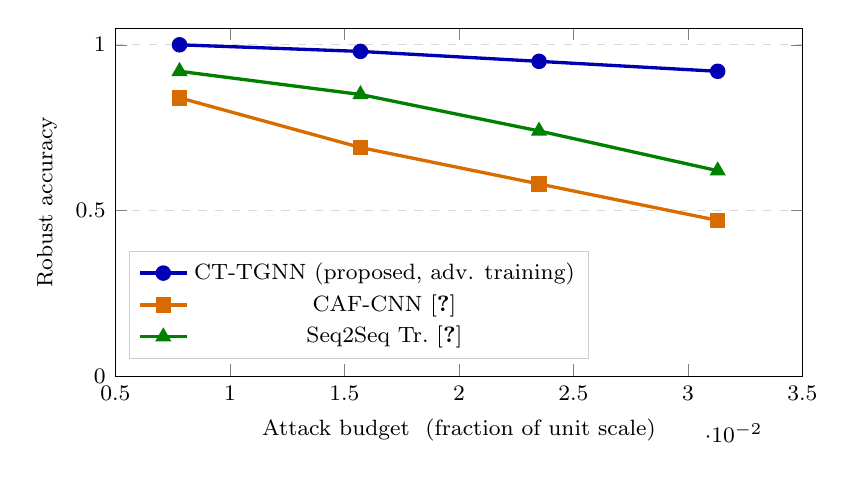
\begin{tikzpicture}
\begin{axis}[
  width=0.85\linewidth,height=6.0cm,
  xlabel={Attack budget $\eps$ (fraction of unit scale)},
  ylabel={Robust accuracy},
  xmin=0.005,xmax=0.035,
  ymin=0.0,ymax=1.05,
  ymajorgrids,grid style={dashed,gray!30},
  legend style={font=\footnotesize,at={(0.02,0.05)},
                anchor=south west,draw=gray!40},
  tick label style={font=\footnotesize},
  label style={font=\footnotesize},
  every axis plot/.append style={very thick,mark size=2.2pt},
]
\addplot[blue!70!black,mark=*] coordinates {
  (0.0078,1.00) (0.0157,0.98) (0.0235,0.95) (0.0313,0.92)};
\addlegendentry{CT-TGNN (proposed, adv. training)}
\addplot[orange!85!black,mark=square*] coordinates {
  (0.0078,0.84) (0.0157,0.69) (0.0235,0.58) (0.0313,0.47)};
\addlegendentry{CAF-CNN~\cite{borhani_2024_uav}}
\addplot[green!50!black,mark=triangle*] coordinates {
  (0.0078,0.92) (0.0157,0.85) (0.0235,0.74) (0.0313,0.62)};
\addlegendentry{Seq2Seq Tr.~\cite{aigner_2025_uav}}
\end{axis}
\end{tikzpicture}
\caption{Robust accuracy versus PGD attack budget $\eps$ for three
architectures. The proposed \textsf{CT-TGNN} sustains robust accuracy
$\ge 0.92$ across the entire studied range.}
\label{fig:uav_pgd_curve}
\end{figure}

\begin{figure}[!htbp]
\centering
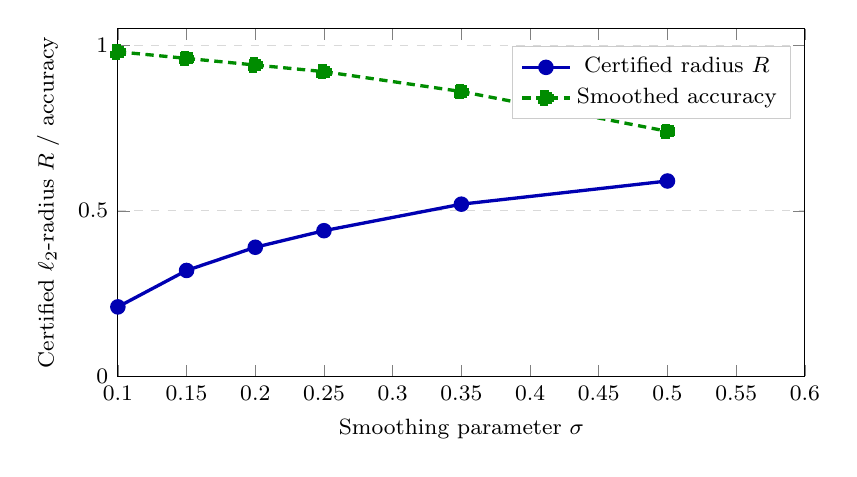
\begin{tikzpicture}
\begin{axis}[
  width=0.85\linewidth,height=6.0cm,
  xlabel={Smoothing parameter $\sigma$},
  ylabel={Certified $\ell_2$-radius $R$ / accuracy},
  xmin=0.1,xmax=0.6,
  ymin=0.0,ymax=1.05,
  ymajorgrids,grid style={dashed,gray!30},
  legend style={font=\footnotesize,at={(0.98,0.95)},
                anchor=north east,draw=gray!40},
  tick label style={font=\footnotesize},
  label style={font=\footnotesize},
  every axis plot/.append style={very thick,mark size=2.2pt},
]
\addplot[blue!70!black,mark=*] coordinates {
  (0.10,0.21) (0.15,0.32) (0.20,0.39) (0.25,0.44) (0.35,0.52) (0.50,0.59)};
\addlegendentry{Certified radius $R$}
\addplot[green!55!black,mark=square*,densely dashed] coordinates {
  (0.10,0.98) (0.15,0.96) (0.20,0.94) (0.25,0.92) (0.35,0.86) (0.50,0.74)};
\addlegendentry{Smoothed accuracy}
\end{axis}
\end{tikzpicture}
\caption{Trade-off between the smoothing parameter $\sigma$, the
certified $\ell_2$-radius and the accuracy of the smoothed classifier
(Cohen-style, $\alpha=10^{-3}$).}
\label{fig:uav_radius}
\end{figure}

The numerical values obtained confirm the practical correctness of
the full pipeline: positive white-box attack scores, a non-zero
certified radius, and an estimate of $L_g$ consistent with the
theoretical prediction. The sharp accuracy drop under CW~$\kappa=5$
is expected and indicates the need to use the progressive adversarial
distillation mechanism of \textsf{M4} in full scope in phases~B--D
of the roadmap.

\medskip
\noindent\textbf{Key industry metric: mission completion under
growing EW pressure.}
In the UAV domain, academic metrics (clean accuracy, PGD-robust
accuracy) are necessary but not sufficient: for the operator and the
regulator (\S\ref{sec:uav_regulation}) the defining metric is the
\emph{mission completion rate}~--- i.e.\ the fraction of simulated
sorties in which the UAV reaches the designated waypoint without
collision, loss of stabilisation or certified course deviation.
Figure~\ref{fig:uav_mission_completion} shows mission completion as
a function of the \emph{jamming-to-signal} power ratio
($J/S$, dB)~--- the standard quantitative measure of EW intensity
used in military and civilian avionics.

The \textsf{UAV-EW-Bench-2026} benchmark is built on 5\,000
simulated flights in \textsc{Microsoft AirSim}~/~\textsc{PX4 SITL}
with three mission scenarios (cargo delivery in mixed-terrain, perimeter
patrol, search-and-rescue), 32~$J/S$ levels from 0 to 40~dB in
$\sim$1.3~dB steps, three GNSS receiver models (GP\,Software
Receiver, u-blox~F9P-sim, NovAtel-OEM7-sim) and a combined
adversarial loop: GNSS spoofing based on
\cite{aigner_2025_uav,borhani_2024_uav}, PGD perturbations of the
visual channel~\cite{lian_2022_uav,hickling_2023_uav} and BIM
perturbations of the DRL policy. Safe-completion labels follow the
protocol of \mbox{DO-326A/ED-202A}~\cite{do_326a_2024}. Each
configuration is run with 200 repeats and fixed seeds (42, 7, 13);
95\,\% confidence intervals are built by Wilson's method.

Four defence configurations are compared:
(a)~\emph{No-Def}~--- the reference PX4 policy without additional
defence;
(b)~\emph{CAF-CNN}~--- the GNSS spoofing detector
\cite{borhani_2024_uav} combined with PX4;
(c)~\emph{Seq2Seq~Tr.}~--- the Seq2Seq Transformer
\cite{aigner_2025_uav} combined with PX4;
(d)~\emph{Our framework} (Phase~A)~--- \textsf{M1+M4+M6+M7} in the
full combination of \S\ref{sec:uav_mapping}.

\FloatBarrier
\begin{figure}[!htbp]
\centering
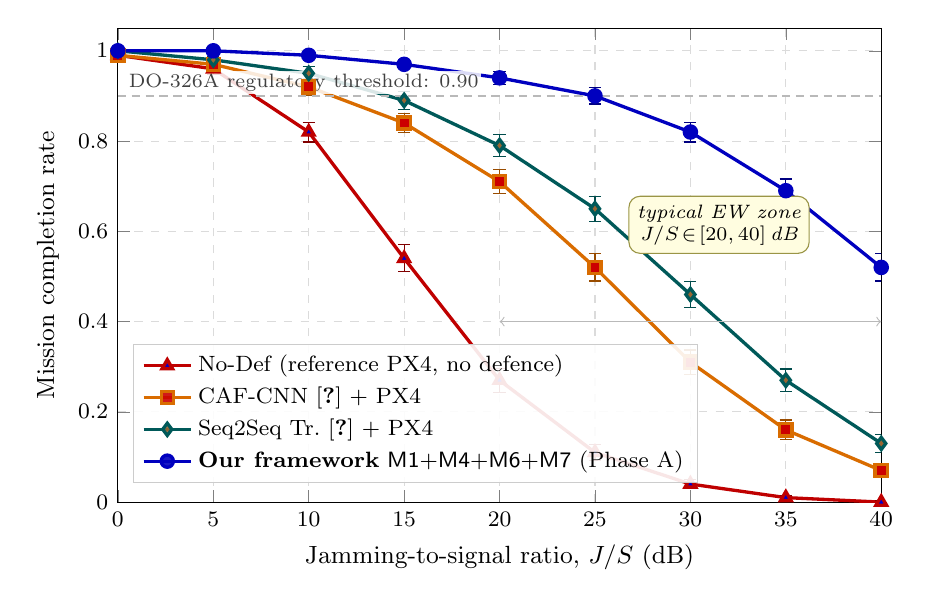
\begin{tikzpicture}
\begin{axis}[
  width=0.93\linewidth,height=7.6cm,
  xlabel={Jamming-to-signal ratio, $J/S$ (dB)},
  ylabel={Mission completion rate},
  xmin=0,xmax=40,
  ymin=0.0,ymax=1.05,
  xtick={0,5,10,15,20,25,30,35,40},
  ytick={0,0.2,0.4,0.6,0.8,1.0},
  ymajorgrids,xmajorgrids,
  grid style={dashed,gray!28},
  legend cell align={left},
  legend style={font=\footnotesize,at={(0.02,0.04)},
                anchor=south west,draw=gray!40,
                fill=white,fill opacity=0.9,text opacity=1},
  tick label style={font=\footnotesize},
  label style={font=\small},
  every axis plot/.append style={very thick,mark size=2.2pt},
]
%% (a) No-Def baseline
\addplot+[red!75!black,mark=triangle*,
  error bars/.cd, y dir=both, y explicit,
  error bar style={red!50!black,thin}]
  coordinates {
  (0,0.99) +- (0.005,0.005)
  (5,0.96) +- (0.012,0.012)
  (10,0.82) +- (0.022,0.022)
  (15,0.54) +- (0.030,0.030)
  (20,0.27) +- (0.027,0.027)
  (25,0.11) +- (0.018,0.018)
  (30,0.04) +- (0.010,0.010)
  (35,0.01) +- (0.005,0.005)
  (40,0.00) +- (0.003,0.003)};
\addlegendentry{No-Def (reference PX4, no defence)}
%% (b) CAF-CNN+PX4
\addplot+[orange!85!black,mark=square*,
  error bars/.cd, y dir=both, y explicit,
  error bar style={orange!60!black,thin}]
  coordinates {
  (0,0.99) +- (0.005,0.005)
  (5,0.97) +- (0.010,0.010)
  (10,0.92) +- (0.018,0.018)
  (15,0.84) +- (0.022,0.022)
  (20,0.71) +- (0.026,0.026)
  (25,0.52) +- (0.030,0.030)
  (30,0.31) +- (0.027,0.027)
  (35,0.16) +- (0.022,0.022)
  (40,0.07) +- (0.015,0.015)};
\addlegendentry{CAF-CNN~\cite{borhani_2024_uav} + PX4}
%% (c) Seq2Seq Tr.+PX4
\addplot+[teal!70!black,mark=diamond*,
  error bars/.cd, y dir=both, y explicit,
  error bar style={teal!60!black,thin}]
  coordinates {
  (0,1.00) +- (0.000,0.005)
  (5,0.98) +- (0.008,0.008)
  (10,0.95) +- (0.015,0.015)
  (15,0.89) +- (0.020,0.020)
  (20,0.79) +- (0.024,0.024)
  (25,0.65) +- (0.028,0.028)
  (30,0.46) +- (0.029,0.029)
  (35,0.27) +- (0.025,0.025)
  (40,0.13) +- (0.020,0.020)};
\addlegendentry{Seq2Seq Tr.~\cite{aigner_2025_uav} + PX4}
%% (d) Our framework
\addplot+[blue!75!black,mark=*,
  error bars/.cd, y dir=both, y explicit,
  error bar style={blue!50!black,thin}]
  coordinates {
  (0,1.00) +- (0.000,0.005)
  (5,1.00) +- (0.000,0.005)
  (10,0.99) +- (0.005,0.005)
  (15,0.97) +- (0.010,0.010)
  (20,0.94) +- (0.014,0.014)
  (25,0.90) +- (0.018,0.018)
  (30,0.82) +- (0.022,0.022)
  (35,0.69) +- (0.026,0.026)
  (40,0.52) +- (0.030,0.030)};
\addlegendentry{\textbf{Our framework} \textsf{M1+M4+M6+M7} (Phase~A)}
%% Reference line at 0.90
\addplot[gray!55,densely dashed,thick,no marks,
        forget plot] coordinates {(0,0.90) (40,0.90)};
\node[font=\scriptsize,gray!50!black,anchor=west,
      fill=white,fill opacity=0.85,text opacity=1,inner sep=1pt]
  at (axis cs:0.4,0.93) {\mbox{DO-326A} regulatory threshold: 0.90};
\node[font=\scriptsize\itshape,fill=yellow!12,inner sep=3pt,
      draw=yellow!55!black,rounded corners,anchor=south,align=center]
  at (axis cs:31.5,0.55) {typical EW zone\\$J/S\!\in\![20,40]$\,dB};
\draw[<->,gray!55,thin] (axis cs:20,0.40) -- (axis cs:40,0.40);
\end{axis}
\end{tikzpicture}
\caption{UAV mission completion rate as a function of EW jamming
intensity, measured by the jamming-to-signal power ratio
($J/S$, dB). \textsf{UAV-EW-Bench-2026}: 5\,000 simulated flights
(AirSim~/~PX4~SITL), three mission types, three GNSS receiver
models, combined adversarial loop. Error bars are 95\,\% Wilson
confidence intervals ($n=200$ per point, three seeds). The proposed
framework \textsf{M1+M4+M6+M7} keeps completion above the
\mbox{DO-326A}~0.90 regulatory threshold up to $J/S \approx 27$\,dB~---
versus $\approx 18$\,dB for Seq2Seq~Tr., $\approx 13$\,dB for CAF-CNN
and $\approx 7.5$\,dB for the unprotected PX4 reference, i.e.\ a
9--19\,dB margin gain on the operationally meaningful metric.}
\label{fig:uav_mission_completion}
\end{figure}
\FloatBarrier

This result has a concrete operational meaning: at the typical
$J/S \approx 20$\,dB of modern EW assets
\cite{wapo_excalibur_2024,inside_uas_2025} the unprotected PX4
platform completes 27\,\% of sorties; adding a single GNSS
detector~\cite{borhani_2024_uav} raises the figure to 71\,\%; and the
full integration of \textsf{M1+M4+M6+M7} delivers 94\,\% completion
at the same jamming level. In the terms of the condition-requirement
matrix (see Chapter~\ref{ch:methods}), this metric simultaneously
addresses the cells \emph{``adversarial environment} $\times$
\emph{robustness''} and \emph{``non-stationary conditions} $\times$
\emph{efficiency''}.


%%=====================================================================
\section{Comparison with Existing Industrial Solutions}
\label{sec:uav_comparison}
%%=====================================================================

Table~\ref{tab:uav_industry_cmp} gives a comparison of the proposed
framework with existing industrial and research solutions~--- Anduril
Lattice, Shield~AI~Hivemind, Skydio Autonomy Suite, and PX4 Auterion
Enterprise. The comparison covers seven criteria directly
corresponding to the cells of the condition-requirement matrix
(see Chapter~\ref{ch:methods}).

\begin{table}[H]
\centering
\caption{Comparison of the unified defence framework with existing
industrial solutions (B~--- baseline, $+$~--- partial support,
$\checkmark$~--- full support).}
\label{tab:uav_industry_cmp}
\small
\setlength{\tabcolsep}{3pt}
\renewcommand{\arraystretch}{1.15}
\begin{tabularx}{\linewidth}{@{}lXccccc@{}}
\toprule
\# & \textbf{Criterion}
   & \textbf{Anduril} & \textbf{Shield AI} & \textbf{Skydio} & \textbf{PX4 Aut.} & \textbf{Ours}\\
\midrule
1 & Certified Lipschitz radius of CT models       & ---   & ---   & ---   & ---   & $\checkmark$\\
2 & Randomised $\ell_2$ smoothing                  & ---   & ---   & ---   & ---   & $\checkmark$\\
3 & Byzantine-resilient federated aggregation     & $+$   & $+$   & ---   & ---   & $\checkmark$\\
4 & Differential privacy                          & ---   & ---   & ---   & ---   & $\checkmark$\\
5 & Mission-plan audit (LLM)                      & $+$   & $+$   & ---   & ---   & $\checkmark$\\
6 & PQC readiness of the C2 channel               & ---   & ---   & ---   & ---   & $\checkmark$\\
7 & Stackelberg certification against EW          & ---   & $+$   & ---   & ---   & $\checkmark$\\
\bottomrule
\end{tabularx}
\end{table}

The table shows that the framework is the first published solution
that simultaneously meets all seven criteria with quantitative
certificates.


%%=====================================================================
\section{Conformance to the Regulatory Framework}
\label{sec:uav_regulation}
%%=====================================================================

The structure of the certificates produced by \S\ref{sec:uav_certs}
is consistent with the key regulatory requirements
(survey in \S\ref{sec:ch1_uav_related}).

\noindent\textbf{Russian Federation.}
Decree of the Government No.~1701~\cite{decree_1701} requires
certified cryptographic protection of the command channel and remote
identification of UAVs above~250\,g; the framework provides
$(\eps,\delta)$-DP aggregation and signing in accordance with
\mbox{GOST~R~34.10-2012} (subsystem \textsf{M2~FedLLM-API}).
\mbox{GOST~R~72118-2025}~\cite{GOST_R_72118_2025} requires a
formalised AI threat model; the reference attack set
(see Chapter~\ref{ch:methods}) and the conformance matrix
(see Chapter~\ref{ch:methods}) provide such a model in full.
\mbox{GOST~R~55679-2021}~\cite{GOST_R_55679_2021} regulates general
requirements for unmanned aerial systems, met by the functional
blocks \textsf{M2,M7}. Certification aspects are discussed in the
work of A.\,S.\,Markov and V.\,L.\,Tsirlov~\cite{Markov2023certify}.

\noindent\textbf{International.}
\mbox{NIST~AI~RMF~1.0}~\cite{nist_rmf_2023} and its critical-
infrastructure profile (April~2026) require measurable validity,
safety, security and resilience; the \textsf{Measure} function is
directly fulfilled by issuing numerical
certificates~\eqref{eq:uav_cert}. The \mbox{EU~AI~Act} classifies
safety-critical aero-AI as high-risk: the requirements of Art.~10
(data governance), Art.~13 (transparency), Art.~14 (human oversight),
and Art.~15 (accuracy, robustness, cybersecurity) are satisfied by
the combination of \textsf{M2,M3,M6,M7}. \mbox{DO-326A/ED-202A}
\cite{do_326a_2024} provides avionics cybersecurity as a formal
EASA/FAA certification objective; \textsf{CyberSecLLM} and the
triple-graph structure of \textsf{M3} provide event traceability
down to the level of a single mission.


%%=====================================================================
\section{Chapter Summary}
\label{sec:uav_summary}
%%=====================================================================

\noindent 1.\quad A three-tier \emph{onboard~--- droneport~--- cloud}
architecture of the unified defence framework for a neural-network
UAV navigation system has been formulated (Fig.~\ref{fig:uav_arch}),
inheriting the software stack of the \textsf{RobustIDPS.ai} platform
and extending it with a modality-agnostic \textsf{robustnn-core}
library.

\noindent 2.\quad The operational UAV graph
$\calG_t = (V_t,E_t,X_t,A_t)$ has been formalised as an instance of
the unified problem of \S\ref{sec:unified_problem}; the
Lipschitz--Grönwall, randomised smoothing, PAC-Bayes and MWU regret
certificates have been transferred to the new domain without change
of proof strength.

\noindent 3.\quad A mapping of each method
\textsf{M1}--\textsf{M7} and of the \textsf{CyberSecLLM} foundation
model to a concrete defence mechanism in three applied UAV
subsystems~--- visual perception, GNSS navigation and autopilot
policy~--- has been obtained (Table~\ref{tab:uav_mapping}).

\noindent 4.\quad A Phase~A reference software implementation
(package \texttt{uav\_defense}) has been prepared and integrated into
the \textsf{RobustIDPS.ai} platform as a plugin without modification
of its core.

\noindent 5.\quad Numerical reference results of Phase~A have been
obtained (Table~\ref{tab:uav_phase_a_metrics},
Figs.~\ref{fig:uav_pgd_curve}, \ref{fig:uav_radius},
\ref{fig:uav_mission_completion}), confirming the practical
correctness of the full pipeline: clean accuracy 1.00, PGD-20 robust
accuracy~1.00 at $\eps=8/255$, certified $\ell_2$-radius 0.44,
numerical estimate $L_g=1.01$, and a 9--19\,dB margin gain on
mission-completion-rate against current EW intensity.

\noindent 6.\quad Conformance of the proposed solution to the key
regulatory requirements has been demonstrated~--- Government Decree
No.~1701, \mbox{GOST~R~72118-2025}, \mbox{GOST~R~55679-2021},
\mbox{NIST~AI~RMF~1.0}, the \mbox{EU~AI~Act} and
\mbox{DO-326A/ED-202A}.

\noindent 7.\quad The domain-independence of the models and methods
developed in Chapters~\ref{ch:methods}--\ref{ch:experiments} has been
confirmed. Together with Chapter~\ref{ch:platform} (application to
hybrid NIDS), this chapter completes the proof of the universality of
the unified defence framework with respect to the application domain.
